\documentclass[a4paper]{article}
\usepackage[utf8]{inputenc}
\usepackage[T1]{fontenc}
\usepackage[pdftex]{graphicx}
\usepackage{fancyhdr}
\usepackage{lscape}
\usepackage{color}
\usepackage{qtree}
\usepackage[english]{babel}
\usepackage{graphicx}
\usepackage[colorinlistoftodos]{todonotes}
\usepackage{listings}
\usepackage{color}
\usepackage{float}
\usepackage{changepage}
\usepackage[margin=1in]{geometry}
\definecolor{codegreen}{rgb}{0,0.6,0}
\definecolor{codegray}{rgb}{0.5,0.5,0.5}
\definecolor{codepurple}{rgb}{0.58,0,0.82}
\definecolor{backcolour}{rgb}{0.95,0.95,0.92}
\usepackage[parfill]{parskip}
 \usepackage{ragged2e}
 \lstdefinestyle{mystyle}{
 	backgroundcolor=\color{backcolour},   
 	commentstyle=\color{codegreen},
 	keywordstyle=\color{magenta},
 	numberstyle=\tiny\color{codegray},
 	stringstyle=\color{codepurple},
 	basicstyle=\footnotesize,
 	breakatwhitespace=false,         
 	breaklines=true,                 
 	captionpos=b,                    
 	keepspaces=true,                 
 	numbers=left,                    
 	numbersep=5pt,                  
 	showspaces=false,                
 	showstringspaces=false,
 	showtabs=false,                  
 	tabsize=2
 }
 
\lstset{
	style=mystyle,
	inputencoding=utf8,
	extendedchars=true,
	literate={á}{{\'a}}1 {ã}{{\~a}}1 {é}{{\'e}}1,
	escapechar=\&
}
\title{Algorithmique et structures de données : Mission 6}
\date{1 décembre 2014}
\author{Groupe 1.2: Ivan Ahad - Jérôme Bertaux - Rodolphe Cambier \\ 
	Baptiste Degryse - Wojciech Grynczel - Charles Jaquet}



\begin{document}
\maketitle
\paragraph{Question 1 (Baptiste Degryse)}
Le graphe étant stocké dans une structure Edge List, il faut retrouver le Vertex dans une liste d'edges, en vérifiant à chaque fois si l'edge ne contient pas un pointer vers le vertex, si oui, il faut retirer l'edge. C'est une opération de complexité temporelle O(m) parce qu'il faut toujours tout vérifier pour ne pas rater d'edge.\\
\begin{center}
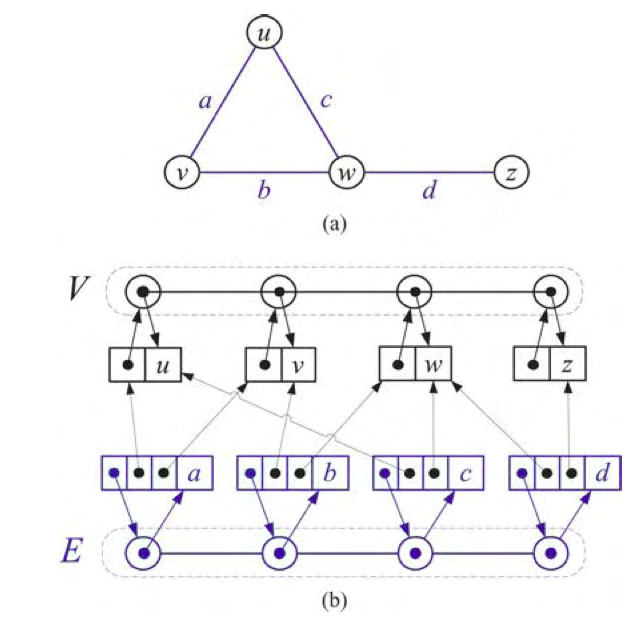
\includegraphics[width=0.8\textwidth]{edgeslist.png}\\
Edge List\\
source: Data Structures and Algorithms in Java Fourth Edition
\end{center}
RemoveEdge est de complexité O(1) puisqu'il s'agit d'une liste doublement chainée, tout comme insertVertex.\\

La réponse dépend bien de la structure de données utilisées pour mémoriser les contenus. Si les edges étaient stockées par vertex, il serait possible d'avoir de bien meilleures performances lors de l'opération removeVertex.\\

Le concept de location aware entry est indispensable pour avoir une complexité O(1) pour la méthode removeEdge.

\paragraph{Question 2}

\paragraph{Question 3}

\paragraph{Question 4}

\paragraph{Question 5}

\paragraph{Question 6 (Charles Jacquet) Quelle est la complexité temporelle de votre algorithme MaxBandWidth(G, a, b) (décrit à la question 5) ? Précisez notamment les hypothèses éventuelles sur l’implémentation des structures de données utilisées, dans la mesure où ces hypothèses seraient importantes pour justifier la complexité annoncée.}



\end{document}
